\section{Testing framework}
This testing framework aims to answer RQ3. The goal is to produce a transparent and sound way of testing core functionality (see section \ref{sec:core-functionality}) performance of any ESB. 
% TODO: vet inte hur du tänkte med ref till lit.rev. men lade en ref till background där de tre sakerna listas.
We have gathered much inspiration from Sanjay \cite{Sanjay2011} regarding what measurements and tests should be performed however an even larger concern of ours is to provide source code and transparency in order for the tests to be repeatable as well as having the ability to discuss how to improve testing which Sanjay misses completely.

\subsection{Measurements}
\label{sec:measurements}
This section will describe what metrics will be collected and why.\\

\begin{table}[H]
	\caption{Metric captured}
	\begin{tabular}{c l}
		\multicolumn{2}{c}{Metrics captured} \\
		\hline
		Client & Response time and throughput \\
		ESB & CPU \\ 
		Web service &  CPU \\
		\hline
	\end{tabular} \\
\end{table}

It is vital to monitor the overall status of all systems involved in the test in order to detect possible chokepoints like network becoming maxed out thus severly limiting the test results.

CPU usage for the web service is important to measure because the web service should not be bottlenecking anything, it is just there to simulate a real back end application and thus has very little to do with ESB testing except for being there as a helper for the whole integrated system.
CPU usage for the ESB is important if two or more ESB solutions are tested against each other for when calculating relative performance where CPU usage relative to how much is processed plays a great part.


\subsubsection{Response time}
The amount of time elapsed since a request was sent to the time a response was received. 
The response time is measured because this is what a single user will be affected by the most, if the response time is very low the user will perceive the system as very fast and vice versa if the response time is too high.

\newpage
\subsubsection{Throughput}
The amount of successful transactions performed per second (tps). A transaction is counted as successful if the response matches expected values.
The value of throughput lies in how many users the system can serve in a specific timeframe. If the throughput is high the system will be able to handle many simultaneous users making the system efficient at handling a high load.

Response time and throughput are the most interesting numbers to investigate as they are very important for end users and systems. 
The more users a system can handle and the faster it does so the higher value the system will get in terms of scalability and performance per processing unit which in turn equals a lower operating cost where the system is able to handle a high amount of users whilst keeping the costs down.

CPU will be measured in order to be able to make sure no hardware limitations occur during testing. 
The CPU on the web service is only collected to make sure that it doesn't act as a bottleneck while testing. 
Although this might not be the case in real world scenarios the aim is not to cap any hardware limitations because that would not give fair test results since the hardware would limit the performance of the system being tested and since the framework is supposed to give the involved system(s) free roam hardware limitations would be in straight contrast to what the framework is about.

\section{Test walktrough}
The tests described below are aimed at measuring the very basic roles of any ESB. 
The tests are very simple with the specific goal of producing a baseline for future tests. 
These basic tests have been chosen since anyone with the development knowledge of an ESB should be able to produce an ESB project capable of delivering a runnable project which exposes these basic funtionalities.

\newpage
\subsection{Pure throughput}
No manipulation of the data will be done by the ESB in this test. The ESB will simply forward all request to the target web service (as fast as possible) (fig.\ref{fig:proxy-diagram}). 
This test could simulate a service where the ESB exposes an inbound endpoint for other an system to connect to, modularizing which service is running in the backend thus giving a separation of concern where the requesting client does not have to know about the responding web service, just that a web service is made available by the ESB.
A comparative test can be performed here as well and that is to not use the ESB which will show what performance impact the ESB adds. 

\begin{figure}[H]
	\centerline{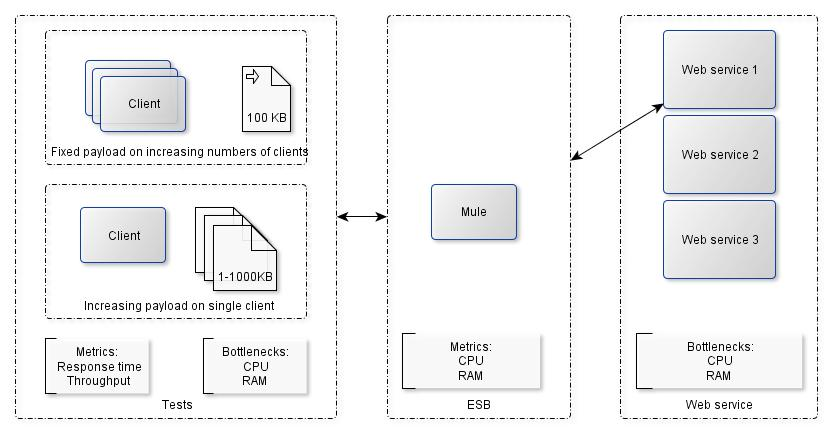
\includegraphics[scale=0.43]{img/direct_proxy}}
	\caption{Direct proxy structural diagram}
	\label{fig:proxy-diagram}
\end{figure}

\newpage
\subsection{Routing}
In this test the ESB will check the incoming request from the Client and dependning on the context, send the request to an appropriate web service which will append some data and return the request to the ESB which will send the response back to the Client (fig.\ref{fig:routing-diagram}).
This represents the ability to have several systems behind an ESB all showing the same front to the clients.
This test is deemed basic because it is what a ESB should do, separate the integrated systems from each other, stepping in as a ``middle-man'' directing requests on behalf of the systems being integrated making the need for changing the systems minimal and just focus on the ESB. 
A test like this could simulate a load balancer where the ESB is a front for two or more systems each running an instance of the same service. Another scenario this could simulate is different systems handling different (but similar) data, for example one system behind the ESB is handling user registrations and another one is handling user logins. The ESB can then look at the request payload and decide what user interaction is happening and thus route the request to the appropriate system.

\begin{figure}[H]
	\centerline{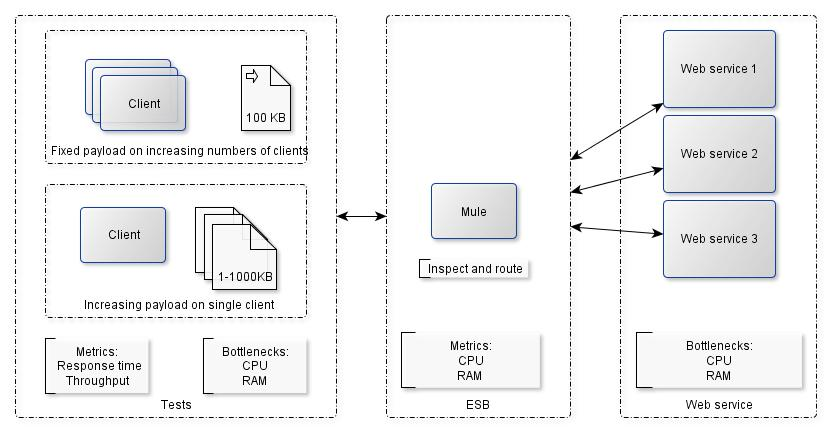
\includegraphics[scale=0.43]{img/Routing}}
	\caption{Routing structural diagram}
	\label{fig:routing-diagram}
\end{figure}

\newpage
\subsection{Message transformation}
The ESB will convert an incoming request to a different protocoll and send it to a web service which will append some data and return the request to the ESB which will transform it back into the format the Client originally sent it (fig.\ref{fig:transform-diagram}).
Transformation is a big deal for any ESB since two systems to be integrated probably won't speak the same language (XML, json etc) and even if they do they may not have the same data format or structure. Of course the systems need to be able to communicate with each others, without an ESB this would become cumbersome since all involved systems would have to be changed in order to understand what the others where saying, just imagine an old system written in COBOL or Assembler and making it communicate with a new system like a web service using REST \cite{whatisrest}. Integration like this cost both money and time and probably won't be future friendly with regards to maintenance.
This could make an ESB invaluable since the ESB would take care of receiving the incoming request in one protocoll, decide where the request is to be sent, transform it to a protocoll which the receiving system can understand, get a response back and transforming it to a protocoll the original system which sent the request will understand and this without even touching the code for the two systems talking to each other.

\begin{figure}[H]
	\centerline{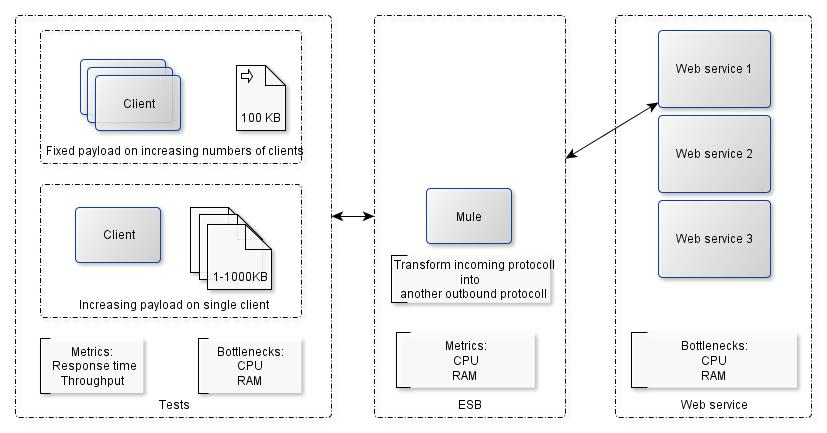
\includegraphics[scale=0.43]{img/transformation}}
	\caption{Transformation structural diagram}
	\label{fig:transform-diagram}
\end{figure}

\newpage
\subsection{Artifacts and tools}
\begin{table}[H]
	\caption{Software and tools}
	\label{table:sw-spec}
	\begin{itemize}
		\item Client: Grinder (v3.8) \cite{whatisgrinder}
		\item ESB: Mule (v3.2.1) \cite{whatismule}
		\item Web service: Jax-WS (v2.2) \cite{whatisjaxws}
		\item OS: Windows 7, 6.1.7600 build 7600
	\end{itemize}
\end{table}

\begin{table}[H]
	\caption{Hardware configuration}
	\label{table:hw-spec}
	\begin{tabular}{c l}
		Component & Specification \\ 
		\hline
		CPU & Intel Core i7 920 @ 2.67GHz  \\
		RAM &  6,00 GB Triple-Channel DDR3 @ 533MHz (7-7-7-20) \\
		Network &  Intel(R) 82567LM-2 Gigabit Network Connection \\
		Motherboard &  Intel Corporation DX58SO (J1PR) \\
		Graphics &  256MB GeForce 7600 GS (MSI) \\
		Hard Drive &  488GB Western Digital WDC WD5001AALS-00L3B2 ATA Device (SATA) \\
		\hline
	\end{tabular} 
\end{table}

In order to minimize the amount of factors that interfere in the tests we recommend having at least three similar state of the art computers, connected to a high-speed network, essential.
It might not be of the greatest importance that the computers are state of the art but in order to not reach a hardware ceiling while testing, such machines are recommended. 
What's most important is that one computer is designated to run ESBs, one is designated to generate traffic(called Client) while the others are simple servers (called Web service) are running a simple application which echoes everything sent to it with an interface using jax-ws to expose the service to soap/XML clients which is the interface used by grinder/the esb to send requests to the web service.

This separating and designating of roles to machines minimizes different hardware affecting test results as the same machines perform the same roles in all tests and the only thing changed is the ESB. 

It also means that if other machines are used in other tests the data produced can be compared to ours and as such validate the data or identify faults in the tests. 
This validation can be done in two ways. 
First is to run the same software versions and compare the results. 
They should be similar deviating only in magnitude. The second way is if using a newer or older software version the values, when put in a graph, will either have the same shape or show areas in which performance has changed, 
if it is the same shape but the magnitude is higher then that is most likely caused by faster machines being used and vice versa if its the same magnitude except in certain areas then that shows an improvement in the software.

The framework is available for others by simply following the base tests described in section \ref{sec:measurements}. Those test can be considered as a basic starting point and expanding these tests with more complicated ones is more than welcome and is encouraged.
The configuration files and all source code used in the framework can be found on github at https://github.com/Datanizze/korsdrag-thesis-files

\subsection{Variables and variable control}
No limitiations has been forseen except for hardware and network.
Hardware and network loads should be monitored so they are not close too 100\% as that would mean there is a major bottleneck present. 
All involved computers running the same operating system.
The three tests have two different focuses. The first is to test scalability with an increasing amount of simulated clients (1, 20, 40, 80, 160, 320) sending concurrent requests with a 100KB payload. 
\subsection{Experiment schedule and execution sequence}
The other is to test load-handling where a single client will send varying sizes of payload, 1KB, 50KB, 100KB, 500KB and 1MB.
\subsection{Validity threats}
This section discusses different validity threats.
\subsubsection{Inefficient code}
We are not expert in the various programming languages and systems used to perform these tests and as such our code might be inefficient and even wrong. Inefficient code is not a problem as long as the same code is used in all tests. Erroneous code however is unmaintainable code and as such will require to be changed in the future and that will most likely affect the test results and test history. 
The possibilities of erroneous code has been limited by focusing the tests on very simple and basic functionality that doesn't require expert knowledge of the ESB in order to get results.
By actually providing the source code we have opened upthe possibility for improvements and additions of more advanced tests which we feel is extremely important for a consistent testing framework used in academia and industry.

\subsection{Misconfigured tools}
Tools such as grinder and our webservice could most certainly be configured better. Especially grinder should be looked at as there are more subtle parameters that can be set that could impact testing results such as sleepTime that pauses the client slightly before sending a new request.

\subsection{Test results and analysis}

This section describes our attempt at running the testing framework with an analysis of the results.
First up is the hardware specification on the five computers used, the scenarios where run with one computer acting as the client , one as the ESB which in this case was mule  and three as web services (see table \ref{table:hw-spec}). 
The computers were connected to an isolated network environment with a 1Gbps speed limit.

As described in table \ref{table:sw-spec}, Grinder was used for simulating clients (users), the ESB in this case was Mule and the web service running on three different computers used JAX-WS.

The results have been obtained by running each test in a period of 5 minutes, that is, 5 minutes for shift in test parameters (changing the number of clients and/or the payload size). 
This showed to be a sufficient amount of time since the amount of requests made in each test ranged from at least 350 to more than 30 000 which was deemed sufficient for liable test results. All data collected in the following sections were done by grinder.

In the following sections the results have been analyzed for each scenario summing it up with an overall analysis of the performed test scenarios.

\subsubsection{Direct proxy results/analysis}
\label{test:results}
The first test for the proxy with a single client sending an increased amount of datai (Fig. \ref{fig:proxy-1-1}). Mule seems to handle this quite well, peaking at about 64 transfers per second (TPS) which could be to be a limit in mule's cxf proxy endpoint which was used. When a single client is sending a very small payload (1KB) it seems like our mule project implementation does not handle this very well since all scenarios where affected by this, limiting the throughput to about two TPS. Mule is handling the direct proxy well and it's handling regular sized payloads with ease only beginning to throttle when the payload size is growing beyond 50KB (Fig. \ref{fig:proxy-2-1}).

\newpage
\begin{figure}[H]
	\caption{TPS for direct proxy.}
	\centerline{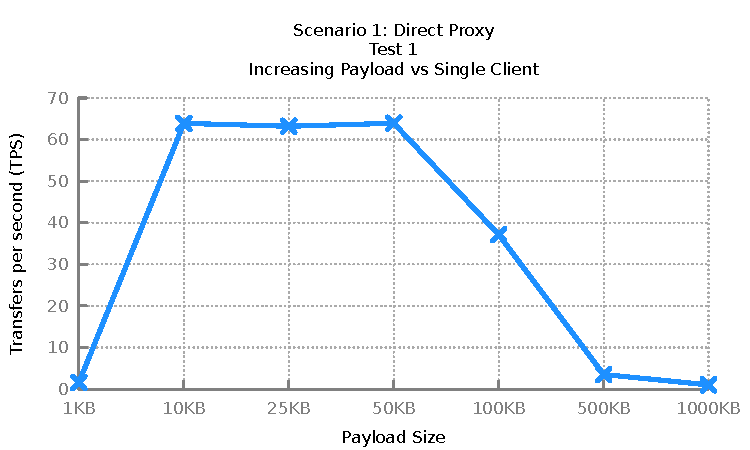
\includegraphics{img/proxy_fu_ip_tps}}
	\label{fig:proxy-1-1}
	As seen in this figure mule is having problems when the single user is sending a small amount (1KB) of data. 
	As the payload increases a bit (10-50KB) a peak at 64 TPS is reached and is then decreased when the payload reaches 100KB.
	When the payload size reaches 500KB mule is having som difficulties keeping up only giving a TPS of 5.

	\caption{Mean response time for direct proxy.}
	\centerline{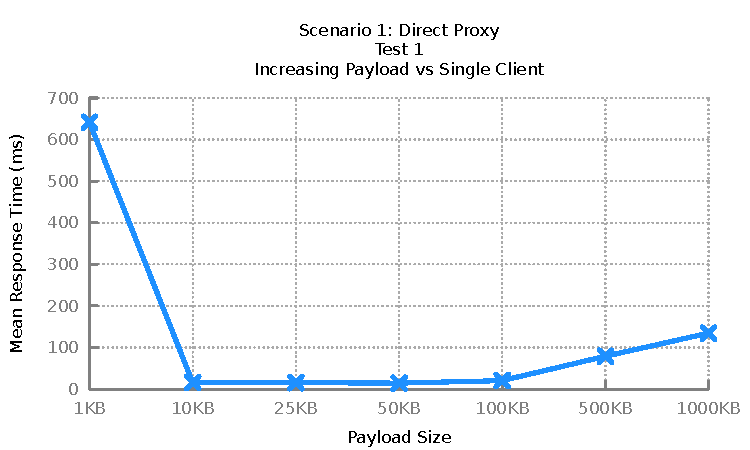
\includegraphics{img/proxy_fu_ip_resp}}
	\label{fig:proxy-1-2}
	The mean response time for the proxy keeps low throughtout the entire test scenario where the largest peak is at the 1KB payload which has been attributed to a limitation or bad configuration in mule.
	It is only when the payload size reaches 500KB and beyond an increase in mean response time occurs.
\end{figure}

\begin{figure}[H]
	\caption{TPS for direct proxy.}
	\centerline{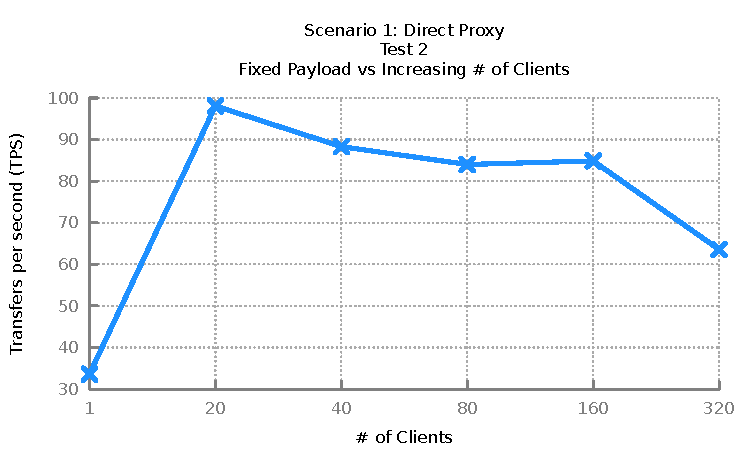
\includegraphics{img/proxy_fp_iu_tps}}
	\label{fig:proxy-2-1}
	Using a fixed payload of 100KB and an increasing number of clients the throughput was peaking at 98 TPS and then decreasing at 320 concurrent users.

	\caption{Mean response time for direct proxy.}
	\centerline{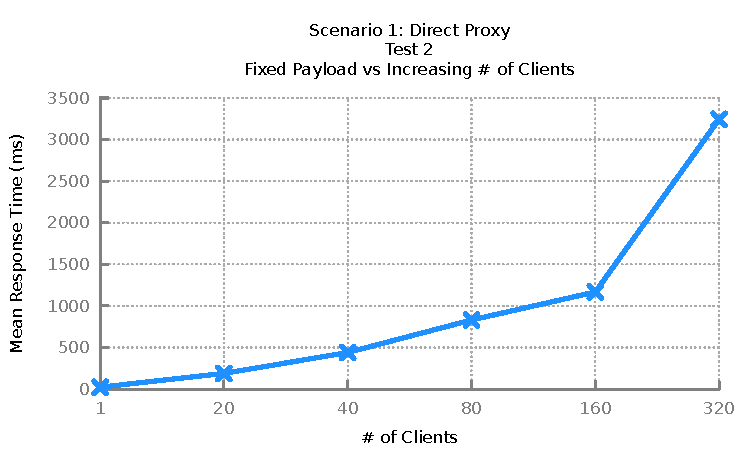
\includegraphics{img/proxy_fp_iu_resp}}
	\label{fig:proxy-2-2}
	 Mule handles the increasing number of clients well, keeping up with a reasonable response time only to slow down when the client count increases beyond 160.
\end{figure}

\begin{figure}[H]
	\caption{TPS for content-based routing.}
	\centerline{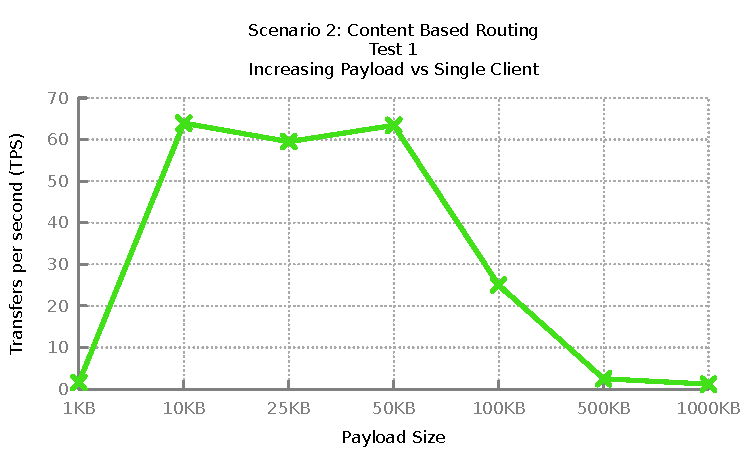
\includegraphics{img/mediation_fu_ip_tps}}
	\label{fig:mediation-1-1}
	As seen here in the content based routing scenario the behavior of mule is similar to the direct proxy (Fig. \ref{fig:proxy-1-1}), starting off slow again at 1KB to increase again at 10-50KB peaking at around 65 TPS and then going down again to about a third in TPS finishing off with 5 TPS at 500KB and 2 TPS at 1MB.

	\caption{Mean response time for content-based routing.}
	\centerline{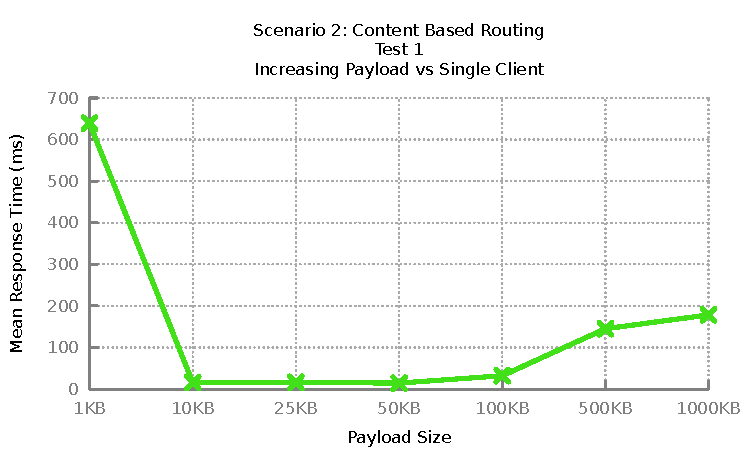
\includegraphics{img/mediation_fu_ip_resp}}
	\label{fig:mediation-1-2}
	Similar to the mean response time seen in the direct proxy scenario (Fig. \ref{proxy-1-2}) with the exception of being slightly higher at 500KB and 1MB caused by the fact that mule has to look at each request and make a decision of which web service to send the request to.
\end{figure}

\begin{figure}[H]
	\caption{TPS for content-based routing.}
	\centerline{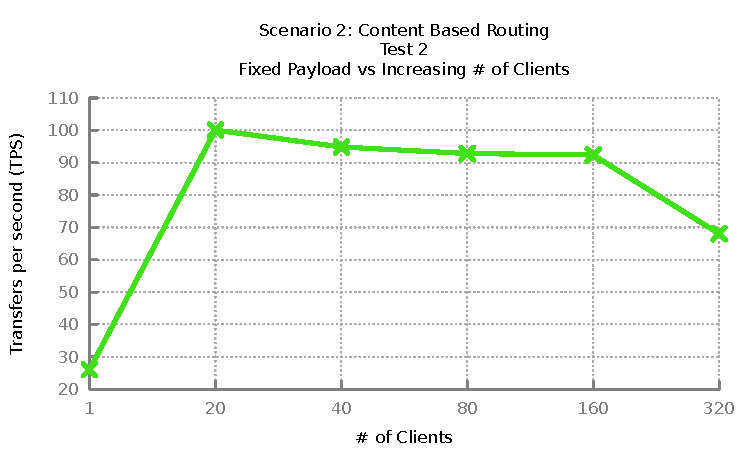
\includegraphics{img/mediation_fp_iu_tps}}
	\label{fig:mediation-2-1}
	As with the direct proxy (Fig. \ref{fig:proxy-2-1}) a single user sending 100KB is limited by the fact that a single user can only send so much requests in a short time frame. The content based routing scenario almost mirrors the direct proxy in this test as would be expected since mule is in addition to proxying just taking a look at a small payload to decide where to send it thus no major processing is done by mule.

	\caption{Mean response time for content-based routing.}
	\centerline{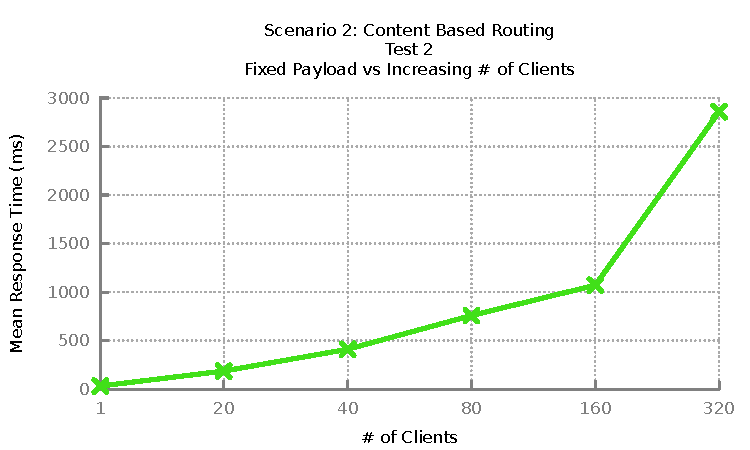
\includegraphics{img/mediation_fp_iu_resp}}
	\label{fig:mediation-2-2}
	The mean response time for this test scenario almost mirrors the same test scenario for the direct proxy (Fig \ref{fig:proxy-2-2}). An almost linear increas in response time can be seen as the number of concurrent users increases only to deviate when the user count peaks at 320 users.
\end{figure}

\begin{figure}[H]
	\caption{TPS for content transformation proxy.}
	\centerline{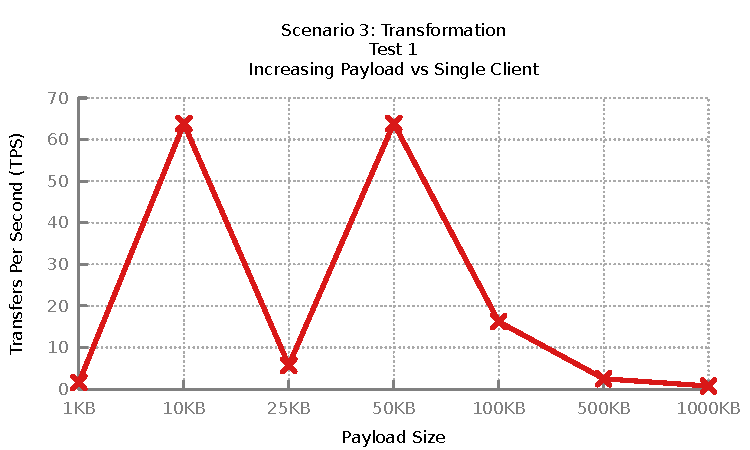
\includegraphics{img/transform_fu_ip_tps}}
	\label{fig:transform-1-1}
	The first test with a single client sending an increasing amount of data in the transformation scenario almost mirrors the direct proxy except for when the client was sending a 25KB data payload. The 25KB part of this test was rerun three times with the same result.
	A conclusion was reached that this might be a bug in the mule software since the throughtput went up again when the payload was increased to 50KB.
	The only other thing noted was a higher decrease in throughput when the payload reached the larger sizes, this was concluded to be caused by mule having a hard time transforming such large amounts of data from json to xml and back again.

	\label{fig:transform-1-2}
	\caption{Mean response time for content transformation proxy.}
	\centerline{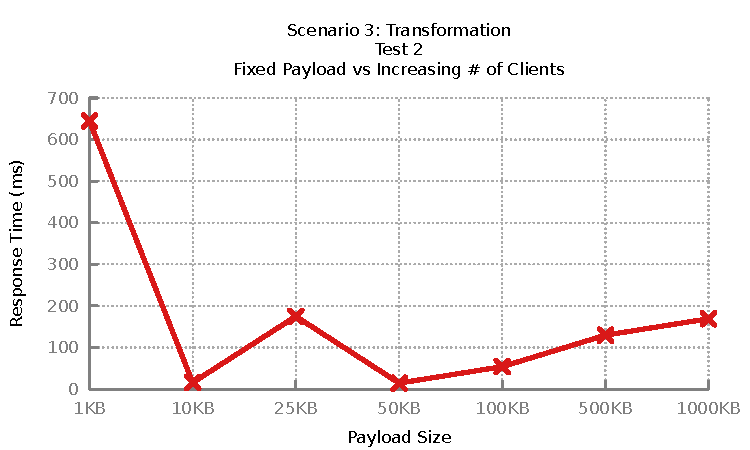
\includegraphics{img/transform_fu_ip_resp}}
	The graph here follows the earlier test scenario graphs (Fig. \ref{fig:proxy-1-2} and \ref{fig:mediation-1-2}) with the exception of the odd 25KB behavior.
\end{figure}

\begin{figure}[H]
	\caption{TPS for content transformation proxy.}
	\centerline{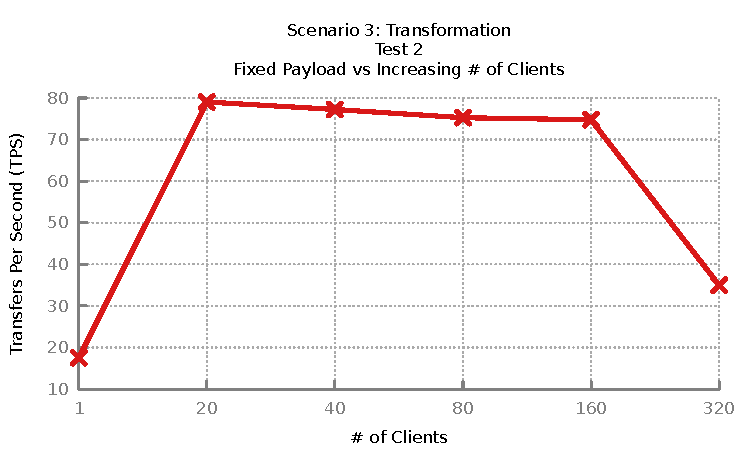
\includegraphics{img/transform_fp_iu_tps}}
	\label{fig:transform-2-1}
	The second test in the transformation scenario shows that sending mule is quite capable of handling transformation of many requests. Note that the throughput is higher for 160 clients with this scenario than in the direct proxy scenario.

	\caption{Mean response time for content transformation proxy.}
	\centerline{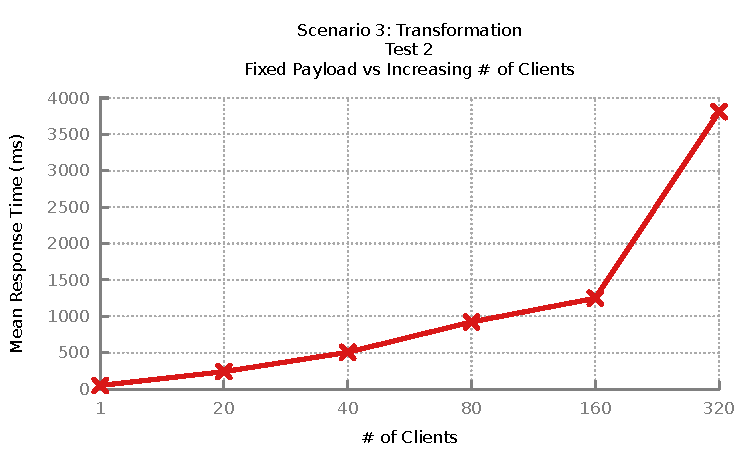
\includegraphics{img/transform_fp_iu_resp}}
	\label{fig:transform-2-2}
	Mule is handling the transformation between JSON and XML well, mirroring the behavior of earlier response time results (Fig. \ref{fig:proxy-2-2} and \ref{fig:mediation-2-2}) when not accounting for magnitude.
\end{figure}

\subsubsection{Overall analysis of performed tests}
\label{sec:test-final-analysis}

The low throughput seen in all of the tests when a single user is sending a very small amount of data (1KB) (Fig. \ref{fig:proxy-1-1}, \ref{fig:-mediation-1-1} and \ref{fig:transform-1-1}) is something we found very strange.
To get som clarity we ran all tests without involving mule, a direct connection between the client (Grinder) and the web service (EchoService). As seen in Figures \ref{fig:direct-1-1}, \ref{fig:direct-1-2}, \ref{fig:direct-2-1}, \ref{fig:direct-2-2} the test results are quite different where the only similar graphs (ignoring magnitude) being the Mean response time.

% something for future work?
No absolute conclusion about what caused the low performance when using mule was reached but we speculated about possible user errors or faulty configurations caused by deficient know-how about coding well-performing mule code.

We decided to run the direct proxy scenario without an ESB in order to see wether the low performance is because of hardware limitations or because of our ESB implementation.

Below are the results from that test followed by an analysis.

\newpage

\begin{figure}[H]
	\caption{TPS for client direct to web service.}
	\centerline{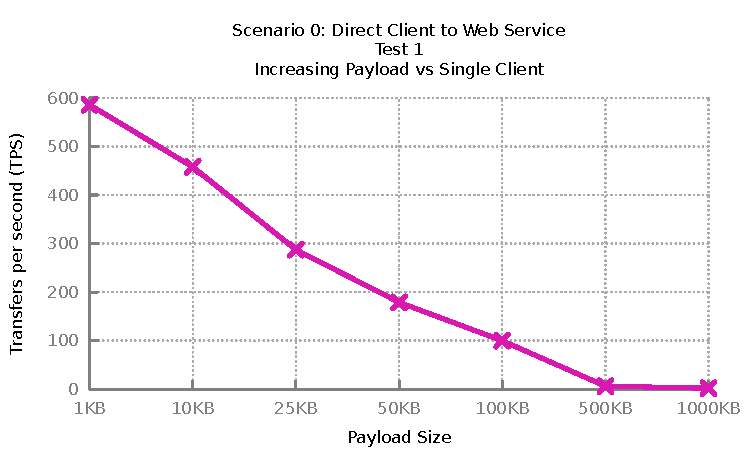
\includegraphics{img/direct_fu_ip_tps}}
	\label{fig:direct-1-1}
	This graph is what one would expect in throughput where a small payload gives a high throughput and a larger payload decreases the throughput.

	\caption{Mean response time for client direct to web service.}
	\centerline{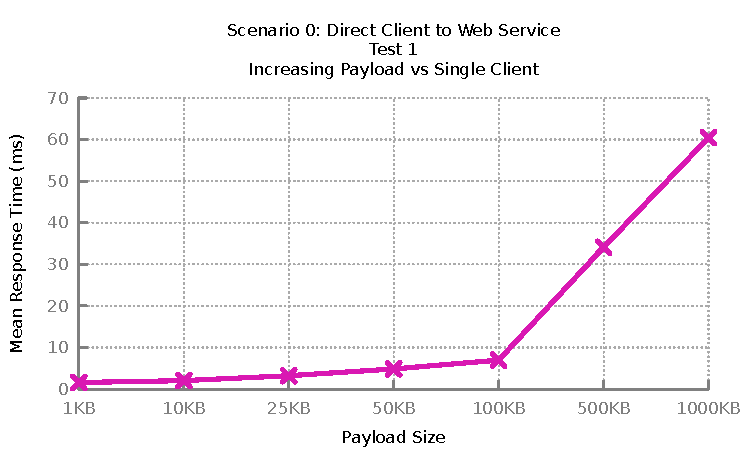
\includegraphics{img/direct_fu_ip_resp}}
	\label{fig:direct-1-2}
	A very good mean repsonse time can be seen here when the payload size is 100KB and below. The response time increased many tenfold after that but is still well below 100ms.
\end{figure}

\begin{figure}[H]
	\caption{TPS for client direct to web service.}
	\centerline{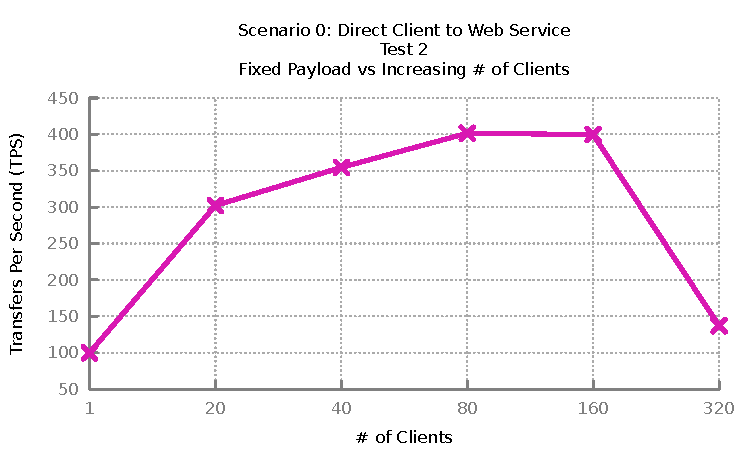
\includegraphics{img/direct_fp_iu_tps}}
	\label{fig:direct-2-1}
	When the test scenario with a fixed payload of 100KB and an increasing amount of users were run we note that a much higher throughput is reached without Mule.
	Running the direct tests with 160+ users sending 100KB requests was throttled by the network, therefore the peak is at approximately 400 TPS. 

	\caption{Mean response time for client direct to web service.}
	\centerline{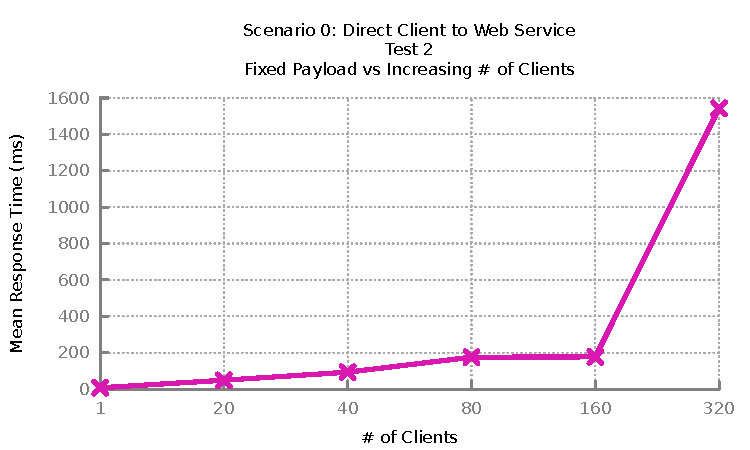
\includegraphics{img/direct_fp_iu_resp}}
	\label{fig:direct-2-2}
	A mean response time below 200ms was kept up until 160 concurrent users. When the user count reached 320 the network got overloaded and thus could not keep up with all requests being sent at a proficient rate making the response time increase by a factor of eight.
\end{figure}

\begin{figure}
	\caption{Average network usage for client direct to web service.}
	\centerline{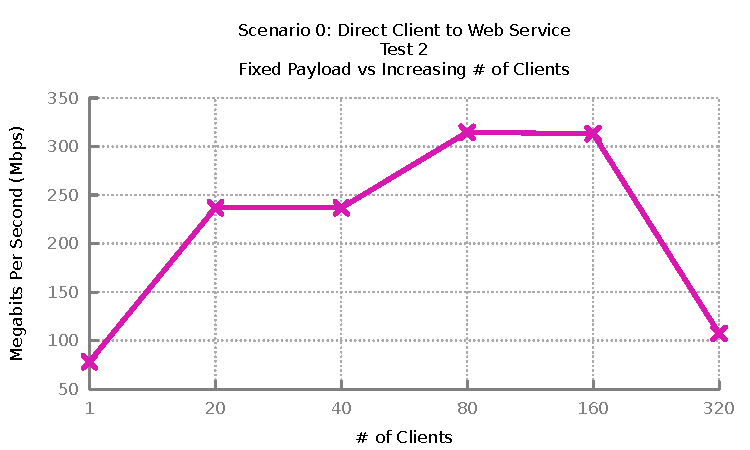
\includegraphics{img/direct_fp_iu_kbs}}
	\label{fig:direct-2-3}
	As seen in this graph the network is peaking at around 320 Megabits per second on average (which is only half the network capacity since the web service is echoing everything sent to it instantly doubling the network load).
\end{figure}

Since the 1 user 1KB test's TPS as shown in figure \ref{fig:direct-1-1} is much higher than in the direct proxy (fig. \ref{fig:proxy-1-1}) our suspicion regarding a limitation/bug in mule seems to fit.

Noting these major differences in test results with and without mule we concluded that it is not necessarily our framework that needs refinement but that our skills programming an integration bus is lacking. This is why our framework matters, everyone won't be able to in a small period of time learn to be masters in each and every ESB being tested. Instead we want to delegate the integration bus part to others with the right competence to integrate with our endpoints (client and web service) in a way that makes optimal use of the ESB. This fits well with the valdity threat about inefficient code in relation to our tests since we are no experts at developing in mule.
